\documentclass[12pt]{article}
\usepackage{amsmath}
\usepackage{tikz}
\usepackage{pgfplots}
\usepackage{float}
\begin{document}
\title{Electrical Engineering 102, Homework 3}
\date{October 25th, 2018}
\author{Michael Wu\\UID: 404751542}
\maketitle

\section*{Problem 1}

\paragraph{a)}

This is not linear. Consider \(x_1(t)=-1\) and \(x_2(t)=1\). Then \(y_1(t)=H(x_1(t))=0\) and \(y_2(t)=H(x_2(t))=2\). If it was linear we have that
\[H(x_1(t)+x_2(t))=H(x_1(t))+H(x_2(t))=y_1(t)+y_2(t)=2\]
But
\[H(x_1(t)+x_2(t))=H(0)=0\]
which is a contradiction.

\paragraph{b)}

This is not linear. If it was linear then
\[y(t)=H(ax(t))=aH(x(t))\]
where \(a\) is a constant. Then letting \(a=0\) we obtain
\[y(t)=H(0)=0\]
But we have that \(H(0)=1\), a contradiction.

\paragraph{c)}

This is not linear. Let \(x^\prime(t)=ax(t)\) where \(a\) is a constant. If it was linear then
\[H(x^\prime(t))=aH(x(t))\]
But
\[H(x^\prime(t)) = \cos(\omega t + ax(t))\]
and
\[aH(x(t))=a\cos(\omega t + x(t))\]
So \(H(x^\prime(t))\neq aH(x(t))\) which is a contradiction.

\paragraph{d)}

This is linear. Let \(x^\prime(t)=ax(t)\) where \(a\) is a constant. Then
\[H(x^\prime(t))=(ax(t)+ax(-t))u(t)=a(x(t)+x(-t))u(t)=aH(x(t))\]
Let there be two functions \(x_1(t)\) and \(x_2(t)\).
Then
\begin{align*}
    H(x_1(t)+x_2(t))&=(x_1(t)+x_2(t)+x_1(-t)+x_2(-t))u(t)\\
    &=(x_1(t)+x_1(-t))u(t)+(x_2(t)+x_2(-t))u(t)\\
    &=H(x_1(t))+H(x_2(t))
\end{align*}
Therefore this system satisfies all the properties necessary to be linear.

\section*{Problem 2}

\paragraph{a)}

\begin{center}
    \begin{tikzpicture}[scale=0.8]
        \begin{axis}[ymin=-0.99,ymax=1.99,xmax=4.99,xmin=-1.99,axis lines = middle]
            \addplot[color=black,mark=none] coordinates {
                (-1,0)
                (0,0.5)
                (1,1.5)
                (2,1.5)
                (3,0.5)
                (4,0)
            };
        \end{axis}
    \end{tikzpicture}
\end{center}

\paragraph{b)}

This system is not time-invariant. We know that
\[u(t)=\sum_{n=0}^\infty \text{rect}\left(t-\frac{2n+1}{2}\right)\]
If the system \(H\) was time-invariant then we would expect that
\begin{align*}
    H(u(t))&=\sum_{n=0}^\infty H\left(\text{rect}\left(t-\frac{2n+1}{2}\right)\right)\\
    &=\sum_{n=0}^\infty y_2(t-n)\\
    &=\sum_{n=0}^\infty e^{-t+n}(u(t-n)-u(t-n-1))
\end{align*}
But we have that
\[H(u(t))=y_1(t)=e^{-t}u(t)\]
and these are not equal, a contradiction.

\section*{Problem 3}

\paragraph{a)}

\begin{enumerate}
    \item Using the flip and drag method we get the following.
    \[y(t)=
        \begin{cases}
            2t^2-8t+8 & 2\leq t < 3\\
            -2t^2+12t-16 & 3\leq t < 4\\
            0 & \text{else}
        \end{cases}
    \]
    This is a parabolic ascent from \(t=2\) to \(t=3\) up to \(2\), then a parabolic descent from \(t=3\) to \(t=4\) from \(2\) to \(0\).
    \item Using the flip and drag method, we get that the convolution is a constant of \(1\) for \(t\leq 1\). Afterwards for \(t\geq 1\) is undergoes
    exponential decay.
    \[y(t)=
        \begin{cases}
            1 & t\leq 1\\
            e^{-t+1} & t>1\\
        \end{cases}
    \]
\end{enumerate}

\paragraph{b)}

\begin{enumerate}
    \item This convolution is an integral that integrates over \(T\) distance prior to the current instance and does no scaling, so \(h(t)=u(t)-u(t-T)\).
    \item This would delay any signal by \(1\), so \(h(t)=\delta(t-1)\).
    \item Given an impulse \(\delta(t)\), this system would cause an infinite number of impulses to happen periodically, so we have
    \[h(t)=\sum_{n=-\infty}^\infty \delta(t-nT_s)\]
\end{enumerate}

\paragraph{c)}

\begin{enumerate}
    \item The left integral becomes \(u(t-1)\). Since convolution is linear, we can take the convolution of this with \(\delta(t-2)\) and \(\delta(2t-8)\) separately and add.
    So the convolution must be \(u(t-3)+u(t-5)\).
    \item We get the following due to linearity.
    \begin{multline*}
        \delta(t-3)*e^{3t}u(-t) + \delta(t-3)*\delta(t+2) + 2*\delta(t-3)\\
        + \delta(t+2)*e^{3t}u(-t) + \delta(t+2)*\delta(t+2) + 2*\delta(t+2)
    \end{multline*}
    Simplifying this term by term yields
    \[e^{3t-9}u(-t+3) + \delta(t-1) + 2 + e^{3t+6}u(-t-2) + \delta(t+4) + 2\]
    which can be rewritten
    \[e^{3t-9}u(-t+3) + e^{3t+6}u(-t-2) + \delta(t-1) + \delta(t+4) + 4\]
    \item First we evaluate \(u(t)*u(t)\).
    \begin{align*}
        u(t)*u(t)&=\int_{-\infty}^\infty u(\tau)u(t-\tau)\, d\tau\\
        &=\begin{cases}
            \int_0^t 1 & t>0\\
            0 & \text{else}
        \end{cases}\\
        &=\begin{cases}
            t & t>0\\
            0 & \text{else}
        \end{cases}\\
        &=r(t)
    \end{align*}
    Then by time invariance and linearity of convolutions we can evaluate the given expression as
    \[\frac{d}{dt}[(u(t)-u(t-1))*u(t-2)]=\frac{d}{dt}(r(t-2)-r(t-3))=u(t-2)-u(t-3)\]
\end{enumerate}

\paragraph{d)}

\begin{enumerate}
    \item This is true. Let us start with the definition of a convolution.
    \[y(t)=\int_{-\infty}^\infty x(\tau)h(t-\tau)\, d\tau\]
    Then we want to find if \(y(-t)=y(t)\) to see if \(y(t)\) is even. We obtain the following.
    \[y(-t)=\int_{-\infty}^\infty x(\tau)h(-t-\tau)\, d\tau\]
    Since \(x(t)\) and \(h(t)\) are odd, we have that \(x(-t)=-x(t)\) and \(h(-t)=-h(t)\). Thus using the substitution \(v=-\tau\) we get
    \begin{align*}
        y(-t)&=-\int_\infty^{-\infty} x(-v)h(-t+v)\, dv\\
        &=\int_{-\infty}^\infty x(-v)h(-(t-v))\, dv\\
        &=\int_{-\infty}^\infty (-x(v))(-h(t-v))\, dv\\
        &=\int_{-\infty}^\infty x(v)h(t-v)\, dv\\
        &=y(t)
    \end{align*}
    We were able to cancel the leading negative by swapping the limits of integration and using the fundamental theorem of calculus. Thus the convolution
    of two odd functions is an even function.
    \item This is false. Consider \(y(t)=u(t)*u(t)=r(t)\), so \(x(t)=u(t)\) and \(h(t)=u(t)\). Then \(y(2t)=r(2t)\). But \(u(2t)*u(2t)=u(t)*u(t)=r(t)\) since \(u(2t)=u(t)\). Thus we have that
    \[y(2t)\neq u(2t)*u(2t)\]
    which should be true if \(y(2t)=h(2t)*x(2t)\). This is a contradiction, so the premise must be false.
\end{enumerate}

\section*{Problem 4}

\paragraph{a)}

\begin{align*}
    h_1(t)&=\int_{-\infty}^{t+t_0} \delta(\tau)\, d\tau\\
    &=u(t+t_0)
\end{align*}
This makes sense because the integral will be \(0\) from \(t=-\infty\) to \(t=-t_0\), after which it will jump up to \(1\).

\paragraph{b)}

\begin{align*}
    h_{\text{eq}}(t)&=\delta(t)*h_1(t) - \delta(t)*h_2(t)*h_3(t)\\
    &=h_1(t)-h_2(t)*h_3(t)\\
    &=u(t+t_0)-u(t-2)*\delta(t-3)\\
    &=u(t+t_0)-u(t-5)
\end{align*}

\paragraph{c)}

\begin{align*}
    x(t)*h_{\text{eq}}(t)&=d(t)*h_{\text{eq}}(t)+2\delta(t-3)*h_{\text{eq}}(t)\\
    &=h_{\text{eq}}(t)+2h_{\text{eq}}(t-3)\\
    &=u(t+t_0)-u(t-5)+2(u(t+t_0-3)-u(t-8))
\end{align*}

\pagebreak

\section*{Problem 5}

\paragraph{a)}

I generated the plot using the following code.
\begin{verbatim}
t=0:0.001:2;
x=2*rectangularPulse(1,2,t);
h=(t-1).*(t>=1).*2.*rectangularPulse(1,2,t);
[conv, times] = nconv(x,t,h,t);
plot(times,conv);
set(gcf,'color','w');
xlabel('t');
ylabel('x(t)*h(t)');
export_fig problem5a.pdf;
\end{verbatim}
\begin{figure}[H]
    \begin{center}
        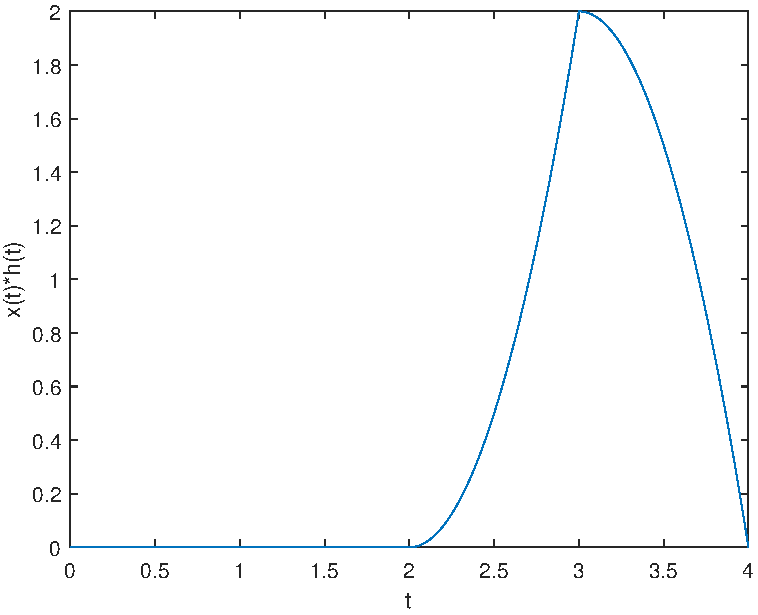
\includegraphics[width=4.5in]{problem5a.pdf}
    \end{center}
\end{figure}

\pagebreak

\paragraph{b)}

I generated the plot using the following code.
\begin{verbatim}
t=-0.5:0.001:0.5;
x=rectangularPulse(t);
[conv, times] = nconv(x,t,x,t);
plot(times,conv);
set(gcf,'color','w');
xlabel('t');
ylabel('rect(t)*rect(t)');
export_fig problem5b.pdf;
\end{verbatim}
\begin{figure}[H]
    \begin{center}
        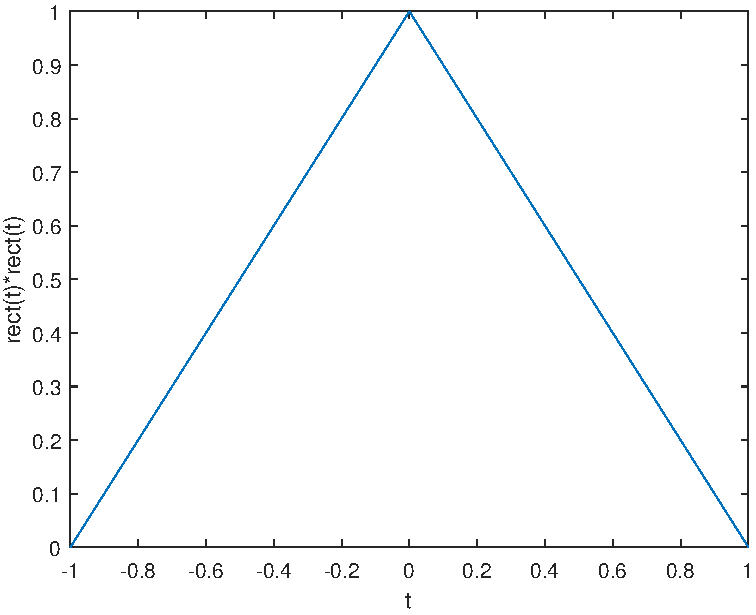
\includegraphics[width=4.5in]{problem5b.pdf}
    \end{center}
\end{figure}

\pagebreak

\paragraph{c)}

I generated the plot using the following code.
\begin{verbatim}
t=-0.5:0.001:0.5;
x=rectangularPulse(t);
[conv, times] = nconv(x,t,x,t);
[conv, times] = nconv(x,t,conv,times);
plot(times,conv);
set(gcf,'color','w');
xlabel('t');
ylabel('rect(t)*rect(t)*rect(t)');
export_fig problem5c.pdf;
\end{verbatim}
\begin{figure}[H]
    \begin{center}
        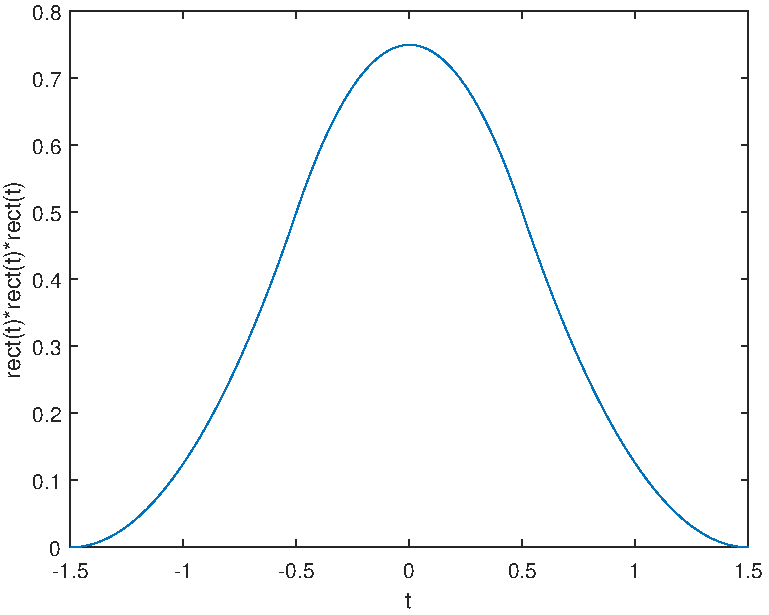
\includegraphics[width=4.5in]{problem5c.pdf}
    \end{center}
\end{figure}

\pagebreak

\paragraph{d)}

I generated the plot using the following code.
\begin{verbatim}
t=-0.5:0.001:0.5;
x=rectangularPulse(t);
[conv, times] = nconv(x,t,x,t);
for i = 0:97
    [conv, times] = nconv(x,t,conv,times);
end
plot(times,conv);
set(gcf,'color','w');
xlabel('t');
ylabel('rect(t)^{100}');
export_fig problem5d.pdf;
\end{verbatim}
\begin{figure}[H]
    \begin{center}
        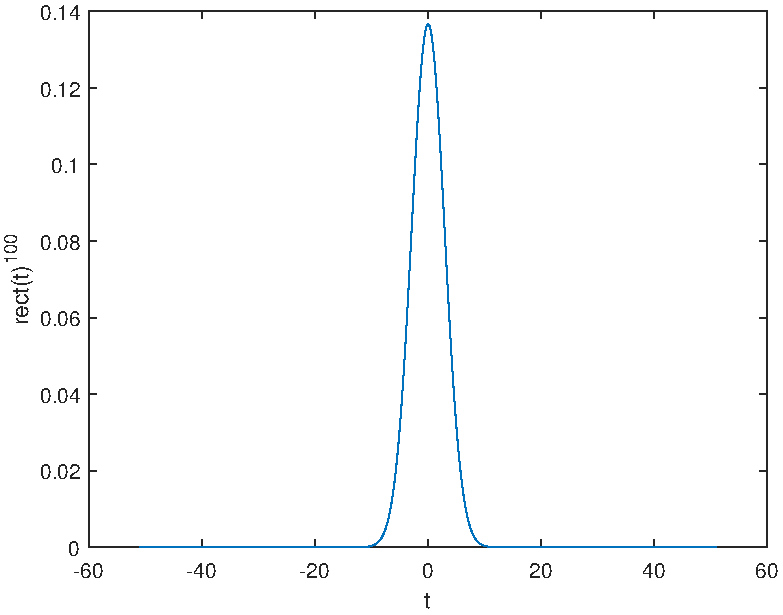
\includegraphics[width=4.5in]{problem5d.pdf}
    \end{center}
\end{figure}

\end{document}